\documentclass[ 12pt, a4paper]{article}
\usepackage[ ]{indentfirst}
\usepackage[ ]{pdflscape}
\usepackage[ ]{graphicx}
\usepackage[ ]{booktabs}
\title{Revisão P2\\Construção de Compiladores\\Prof. Bráulio de Mello}
\author{Erickson G. Müller}
\date{11 de junho de 2026}

\begin{document}
\maketitle
\section*{Conteúdos}
	\begin{itemize}
		\item
	\end{itemize}
\newpage

\section{Tradução dirigida por sintaxe}
\begin{itemize}
	\item $AS \to $ tradução
	\begin{itemize}
		\item código
			\begin{itemize}
				\item operações básicas
				\item mesmo nível
			\end{itemize}
		\item interpretação
		\item ações semânticas
		\item add dados TS
		\item tratamento de erro
	\end{itemize}
\end{itemize}
	\subsection{Árvore de derivação anotada}

	Atributos associados aos símbolos.\\
	\textbf{Exemplo:}\\
		$D::= var: T$\\
		$T::= real$\\
		$T'::= int$\\
		\\
		Ações semânticas:\\
		$\{$add $TS(var.nome, T.tipo)\}$\\
		$\{T.tipo='r'\}$\\
		$\{T.tipo='i'\}$\\
		\\
		$_{var.nome=x_1}$\\
		$_{T.tipo = 'r'}$\\
		cadeia: $x_1:real$

\begin{verbatim}
	TS
	___________________________________
	| x1, r

\end{verbatim}
	\subsection{Esquemas de tradução}

		Esquemas de tradução é o conjunto de ações semânticas
	\begin{itemize}
		\item extensão da GLC
		\item atributos
			\begin{itemize}
				\item sintetizados
				\item herdados
			\end{itemize}
		\item ações semânticas
		\item grafo de dependência
			\begin{itemize}
				\item ordenação uso atributos
			\end{itemize}
		\item passos
			\begin{itemize}
				\item Análise sintática
				\item Árvore de derivação (anotada)
				\item grafo de dependência
			\end{itemize}
	\end{itemize}
	
	\textbf{Exemplo 2:}\\
	$E::=TR$\\
	$R::= Op$ $T \{$print $(Op.simbolo)\}$ $R|E$\\
	$T::= num$ $\{$print $(num.lexval)\}$\\
	\begin{center}
	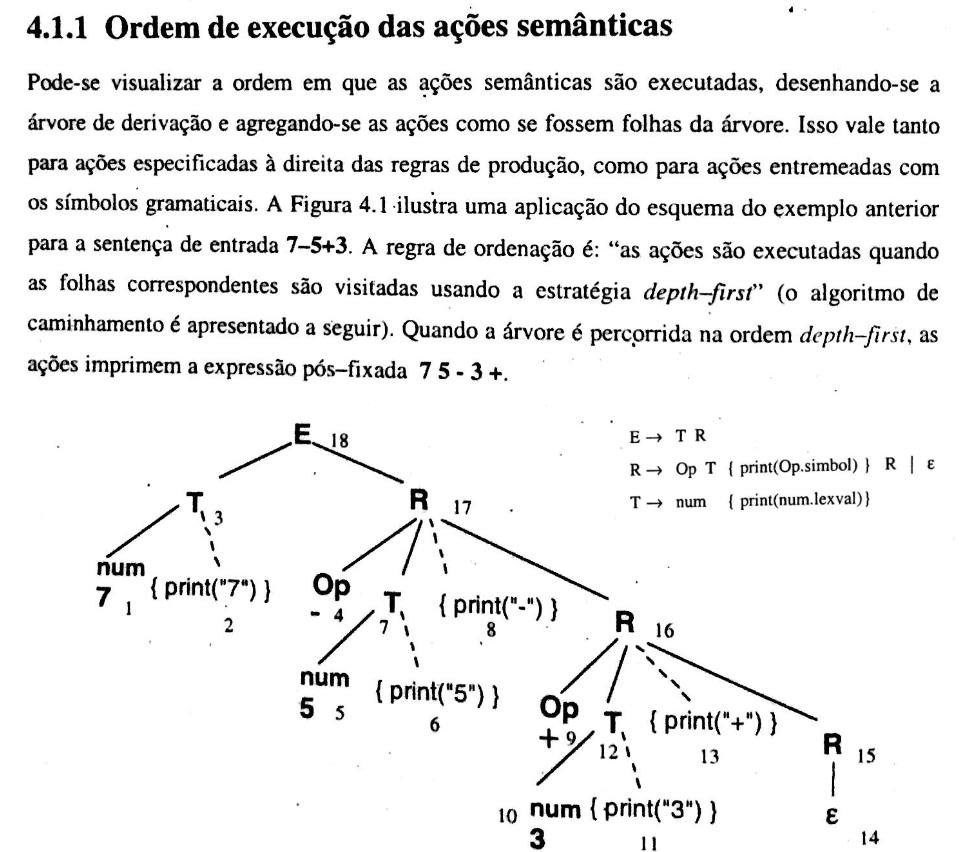
\includegraphics[scale=0.5]{images/arvore-traducao.png}\\
	\end{center}
	A aula seguiu explicando o exemplo da página 7 do fragmento do livro no arquivo \textit{3\_material...} que está no repositório.

\begin{verbatim}
Na GLC:
- Adicionar as produções:
		E::= E-T
		T::= T/F
	e respectivas ações semânticas

- Reconhecer a cadeia:
	8+((6/2-1)+2)=
----------------------------------------
GLC:            Ações semânticas:
	L::= E=  				{print (E.val)}
	E::= E1+T 			{E.val = E1.val + T.val}
	E::= T   				{E.val = T.val}
	T::= T1*F 			{T.val = T1.val * F.val}
	T::= F   				{T.val = F.val}
	F::= (E)  			{F.val = E.val}
	F::= id	  			{F.val = id.lexval}
	E::= E-T  			{E.val = E1.val - T.val}
	T::= T/F  			{T.val = T1.val / F.val}

	
	
Árvore:







E           |
|           |
id.        id.   id.   id.         id.         id.   id.         id.   id.
lex        lex   lex   lex         lex         lex   lex         lex   lex
=8         =(    =(    =6          =2          =1    =)          =2    =)
|           |     |     |           |           |     |           |     |
8     +     (     (     6     /     2     -     1     )     +     2     )     =
\end{verbatim}

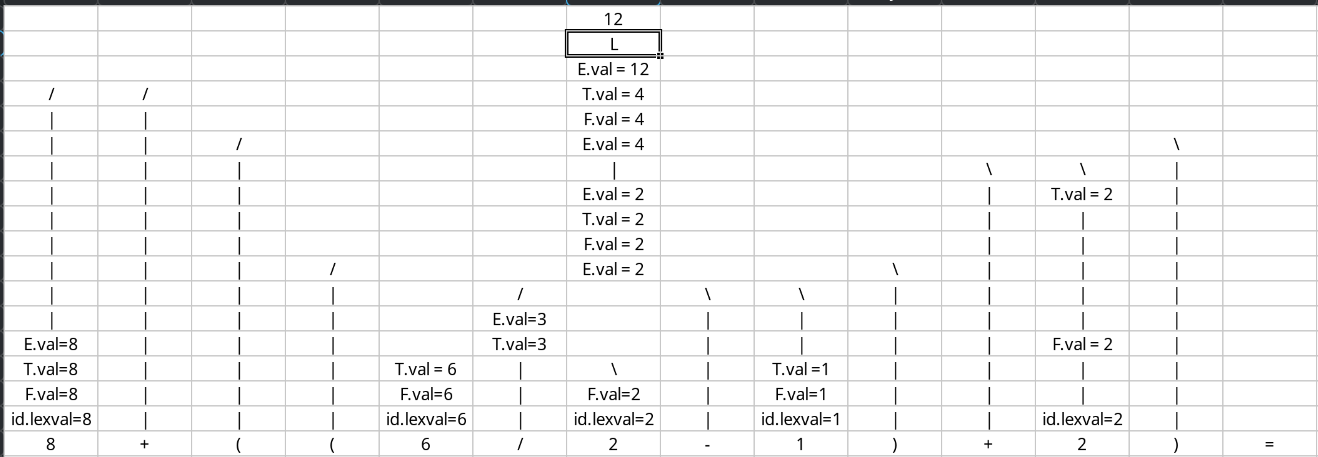
\includegraphics[scale=0.4]{images/arvore-calculadora.png}\\
\end{document}
